\documentclass[11pt,a4paper]{report}
\usepackage[portuges]{babel}
\usepackage[utf8]{inputenc} % define o encoding usado texto fonte (input)--usual "utf8" ou "latin1
\usepackage{graphicx} %permite incluir graficos, tabelas, figuras
\usepackage{subcaption}
\usepackage[title]{appendix}
\usepackage{listings}
\usepackage{color}
\usepackage{multicol}
\usepackage{indentfirst}
\usepackage{hyperref}
\usepackage{amsmath}
\usepackage{amssymb}
\usepackage{float}
\usepackage{enumerate}
\usepackage[shortlabels]{enumitem}
\usepackage[T1]{fontenc}
\usepackage{hyperref}
\usepackage{markdown}



\definecolor{mygreen}{rgb}{0,0.6,0}
\definecolor{mygray}{rgb}{0.5,0.5,0.5}
\definecolor{mymauve}{rgb}{0.58,0,0.82}

\hypersetup{
    colorlinks=true,
    linkcolor=blue,
    urlcolor=black,
    }
    
    
    
\usepackage{bera}% optional: just to have a nice mono-spaced font

\definecolor{eclipseStrings}{RGB}{42,0.0,255}
\definecolor{eclipseKeywords}{RGB}{127,0,85}

\lstdefinelanguage{json}{
    basicstyle=\normalfont\ttfamily,
    commentstyle=\color{eclipseStrings}, % style of comment
    stringstyle=\color{eclipseKeywords}, % style of strings
    numbers=left,
    numberstyle=\scriptsize,
    stepnumber=1,
    numbersep=8pt,
    showstringspaces=false,
    breaklines=true,
    frame=lines,
    backgroundcolor=\color{white}, %only if you like
    string=[s]{"}{"},
    comment=[l]{:\ "},
    morecomment=[l]{:"},
    literate=
        *{0}{{{\color{numb}0}}}{1}
         {1}{{{\color{numb}1}}}{1}
         {2}{{{\color{numb}2}}}{1}
         {3}{{{\color{numb}3}}}{1}
         {4}{{{\color{numb}4}}}{1}
         {5}{{{\color{numb}5}}}{1}
         {6}{{{\color{numb}6}}}{1}
         {7}{{{\color{numb}7}}}{1}
         {8}{{{\color{numb}8}}}{1}
         {9}{{{\color{numb}9}}}{1}
}
    

\lstset{ %
  backgroundcolor=\color{white},   % choose the background color
  basicstyle=\footnotesize,        % size of fonts used for the code
  breaklines=true,                 % automatic line breaking only at whitespace
  captionpos=b,                    % sets the caption-position to bottom
  commentstyle=\color{mygreen},    % comment style
  escapeinside={\%*}{*)},          % if you want to add LaTeX within your code
  keywordstyle=\color{blue},       % keyword style
  stringstyle=\color{mymauve},     % string literal style
}



\title{PLC - Trabalho Prático 1\\
	\large Grupo nº15}

\author{Tomás Vaz de Carvalho Campinho \\ (A91668) \and Miguel Ângelo Alves de Freitas \\ (A91635)
         \and Pedro Alexandre Silva Gomes \\ (A91647)
       } %autores do documento
       
\date{\today} %data

\begin{document}
	\begin{minipage}{0.9\linewidth}
        \centering
		
\includegraphics[width=0.4\textwidth]{um.jpg}\par\vspace{1cm}
		\href{https://www.uminho.pt/PT}
		{\scshape\LARGE Universidade do Minho} \par
		\vspace{0.6cm}
		\href{https://lcc.di.uminho.pt}
		{\scshape\Large Licenciatura em Ciências da Computação} \par
		\maketitle
		\begin{figure}[H]
			
\includegraphics[width=0.32\linewidth]{Tomas.jpg}
			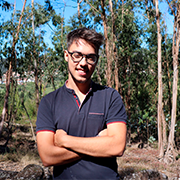
\includegraphics[width=0.32\linewidth]{miguel.png}
			
\includegraphics[width=0.32\linewidth]{pedro.jpg}
		\end{figure}
	\end{minipage}
	
	\tableofcontents
	
	\pagebreak
	
	\chapter{Introdução do problema}
%	
	Este projeto consistiu no desenvolvimento de um processador de inscritos numa atividade desportiva de forma a pôr em prática os conhecimentos adquiridos ao longo das aulas. Para este projeto estão definidos os seguintos objetivos

    \begin{enumerate}[a.]
        \item imprimir o nome e o email dos concorrentes inscritos entre a 5º e a 15º posições.
        \item imprimir o nome dos concorrentes que se inscrevem como 'Individuais' e são de 'Valongo'.
        \item imprimir o telemóvel e a prova em que está inscrito cada concorrente cujo nome seja 'Paulo' ou 'Ricardo', desde que seja da Vodafone.
        \item imprimir os 20 primeiros registos com os nomes convertidos para minúsculas.
        \item imprimir os 20 primeiros registos num novo ficheiro de output mas em formato Json.
    \end{enumerate}
	
	\pagebreak
	\chapter{Resolução/abordagem ao problema}
	\section{Ficheiro inscritos.txt}
	Para o nosso trabalho foi dado como material o ficheiro "inscritos.txt", de forma a conseguirmos testar os nossos programas/funções.
	Para isso primeiramente vimos como é que o ficheiro estava elaborado, percebemos que estava elaborado em forma de tabela, e constatamos o seguinte:
	\begin{itemize}
	    \item Na primeira linha do ficheiro temos o título da tabela
	    \item Na segunda linha do ficheiro temos os rótulos das colunas separados tabs('\textbackslash t')
	    \item Da terceira linha até à ultima vão sendo enumeradas as pessoas inscritas, e cada linha vai ser do tipo: nome \textbackslash t +email \textbackslash t +situação \textbackslash t+data \textbackslash t+tipo\textunderscore inscricao \textbackslash t+valor \textbackslash  +tipo\textunderscore pagamento \textbackslash +......
	\end{itemize}
	\subsection{Exemplo de visualização}
	
	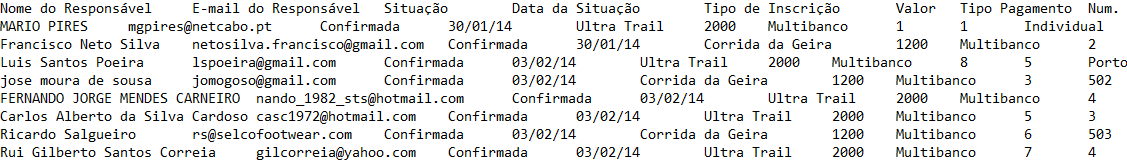
\includegraphics[width=\textwidth]{exemplo inscirtos.png}
	
\pagebreak

	\section{Alinea (a.)}
	\subsection{Problema}
	"Imprimir o nome e o email dos concorrentes inscritos entre a 5º e a 15º posições."
	
	\subsection{Resolução/abordagem}
	Para imprimir o nome e o email dos concorrentes inscritos, entre a 5º e a 15º, posições foi necessário utilizar um intervalo de $[6 - 16]$ devido à ocupação da primeira linha do ficheiro $"inscritos"$ com a identificação dos dados.
    Utilizamos as funções:

    $re.search(pattern, string, flags=0)$ (procura os caracteres de correspondências da String do $pattern$ da expressão regular e retorna $None$ se não encontrar a ocorrência)

    $re.match(pattern, string, flags=0)$ (procura a primeira ocorrência na String do $pattern$ da expressão regular e retorna $None$ se não encontrar a ocorrência) 

    As expressões regulares utilizadas como filtro de pesquisa para cada linha foram:

[\^{} \textbackslash t]+ (reconhece tudo o que está antes do primeiro $tab$)  

\textbackslash t.+@[a-z.]+\textbackslash t (reconhece tudo após o primeiro $tab$ até ao @ e tudo após este até ao próximo $tab$)

Fizemos ainda a separação das ER's por groups para facilitar as utilizações posteriormente necessárias.
	
    
	
	\subsection{Código}
	\begin{lstlisting}[language=python]
    import re

    inscritos = open("inscritos.txt")

    min = 6 
    max = 16                        

    for i, linha in enumerate(inscritos):
        if (i in range(min, max+1)):
            nome = re.match(r'[^\t]+', linha)
            email = re.search(r'\t.+@[a-z.]+\t', linha) 
            if(nome and email):
                print(nome.group(), email.group())
    \end{lstlisting}
    
    \subsection{Output}

	\begin{verbatim}
FERNANDO JORGE MENDES CARNEIRO 	nando_1982_sts@hotmail.com	
Carlos Alberto da Silva Cardoso 	casc1972@hotmail.com	
Ricardo Salgueiro 	rs@selcofootwear.com	
Rui Gilberto Santos Correia 	gilcorreia@yahoo.com	
José Moreira 	jmoreiracdf@gmail.com	
Hélder Silva 	helder.santos.silva@hotmail.com	
JOSE COELHO 	rota_pontual@sapo.pt	
paulo de castro rocha 	pcastrorocha@gmail.com	
Artur Bernardo 	ajbernardo@netcabo.pt	
J Paulo Marques 	pmarques269@gmail.com	
Bruno Manuel Henriques Maceda 	macedobruno10@gmail.com	
    \end{verbatim}

\pagebreak

\section{Alinea (b.)}
	\subsection{Problema}
	"Imprimir o nome dos concorrentes que se inscrevem como 'Individuais' e são de 'Valongo'."
	
	\subsection{Resolução/abordagem}
	
	A estratégia que escolhemos utilizar neste problema consistiu em ler o ficheiro "inscritos.txt", como habitualmente iremos fazer, de seguida, linha a linha fomos procurar ("search") se existir ou não as palavras 'Individual' e 'Valongo' nessa mesma linha, guarda assim a linha em variaveis x e y respetivamente. De seguida vamos dar match ao nome.
	Por último falta validar, ou seja, caso tenho encontrado a palavra Individual e Valongo e pertençam à mesma linha, vai buscar o nome desse grupo e vai imprimir.
    
	
	\subsection{Código}
	\begin{lstlisting}[language=python]
    import re

    inscritos = open("inscritos.txt")

    for linha in inscritos:
        x = re.search(r'(?:Individual)', linha)
        y = re.search(r'(?:Valongo)', linha)
        nome = re.match(r'[^\t]+', linha) #[^\t]+ -> inicio até \t
        if(x and y and nome):
            print(nome.group())
    \end{lstlisting}
    
    \subsection{Output}

	\begin{verbatim}
Vera Cristina Moreira Delgado
Paulo Domingues
Dulce Moreda	
    \end{verbatim}

\pagebreak

    \section{Alinea (c.)}
	\subsection{Problema}
	"imprimir o telemóvel e a prova em que está inscrito cada concorrente cujo nome seja 'Paulo' ou 'Ricardo', desde que seja da Vodafone."
	
	\subsection{Resolução/abordagem}
	A estratégia que escolhemos utilizar neste problema consistiu em ler o ficheiro "inscritos.txt", como habitualmente iremos fazer, para realizar a impressão do número de telemóvel Vodafone (91) e a prova em que está inscrito cada concorrente cujo o primeiro nome seja 'Paulo' ou 'Ricardo', foi necessário as expressões regulares:


    $(?i:Ricardo)$ e $(?i:Paulo)$ (Procuram as primeiras ocorrências das Strings com caracteres maiúsculos e minúsculos)

    $91[0-9]{7}$ (Procura os números de telemóvel que começam em 91)

    $(([0-9]{2}/*){3})(([\textbackslash t ]|[A-z])+)$ (Procura as ocorrências da data do tab e da String posterior, utilizando a separação com groups foi possível escolher apenas a prova que era a String pretendida)
	
	\subsection{Código}
	\begin{lstlisting}[language=python]
    import re

    inscritos = open("inscritos.txt")

    for linha in inscritos:
        x = re.match(r'(?i:Paulo)', linha) #consideramos concorrente cujo *primeiro* nome seja 'Paulo' (PERGUNTAR AO STOR)
        y = re.match(r'(?i:Ricardo)', linha) #consideramos concorrente cujo *primeiro* nome seja 'Ricardo'

    num = re.search(r'91[0-9]{7}', linha) #consideramos Vodafone os números que começam em '91'
    prova = re.search(r'(([0-9]{2}\/*){3})(([\t ]|[A-z])+)', linha) #procuramos a data e o texto seguinte que corresponde a prova
    if((x or y) and num and prova):
        print(num.group(), prova.group(3)) #dividimos em groups e escolhemos o group do nome da prova
    \end{lstlisting}
    
\pagebreak

    \subsection{Output}

	\begin{verbatim}
914465667 	Ultra Trail	
917067362 	Ultra Trail	
917300483 	Ultra Trail	
917804565 	Corrida da Geira	
917364824 	Corrida da Geira	
919597737 	Ultra Trail	
917437387 	Ultra Trail	
919947570 	Ultra Trail	
914536925 	Ultra Trail	
919121762 	Corrida da Geira	
    \end{verbatim}
    
    
\pagebreak

    \section{Alinea (d.)}
	\subsection{Problema}
	" imprimir os 20 primeiros registos com os nomes convertidos para minúsculas.."
	
	\subsection{Resolução/abordagem}
	Para imprimir os 20 primeiros registos com os nomes convertidos para minúsculas, utilizamos o intervalo $[2-21]$ e as funções:

$re.sub(pattern,repl,string,count=0,flags=0)$ (substitui a String separando o  $\n$  da informação final)

$re.split(pattern,string,maxsplit=0,flags=0)$  (divide a String com  tab )

$list(dict.fromkeys(lista))$  (Remove a informação repetida em cada linha)

$join(lista)$ (Junta todos os itens de um dicionário para uma string usando um "\textbackslash t" como separador)

As expressões regulares usadas foram:

\\n e \textbackslash t (Utilizado no split e no sub como referido)

([\^{} \textbackslash t]+)(.+) (Procura a ocorrência antes do primeiro  tab  e do restante da lista para poder separar a String do nome num group e retornar esta em minúsculas)
    
	
	\subsection{Código}
	\begin{lstlisting}[language=python]
    import re

    inscritos = open("inscritos.txt")

    min = 2
    max = 21   

    for i, linha in enumerate(inscritos):
        if(i in range(min, max+1)):
        new_line = re.sub(r'\n', '\t\n', linha) #separar o \n da informação final
        lista = re.split(r'\t', new_line)
        lista = list(dict.fromkeys(lista)) #remover informação repetida
        x = '\t'.join(lista)
        x = re.match(r'([^\t]+)(.+)', x)
        if(x):
            print(x.group(1).lower(), x.group(2))
    \end{lstlisting}
    
    \subsection{Output}
        Output em \hyperlink{Anexo D}{"Anexo D"}
    
        
    

\pagebreak

    \section{Alinea (e.)}
	\subsection{Problema}
	"Imprimir os 20 primeiros registos num novo ficheiro de output mas em formato Json."
	
	\subsection{Resolução/abordagem}
    
	
	\subsection{Código}
	\begin{lstlisting}[language=python]
    import re

    inscritos = open("inscritos.txt")
    ficheiro = open("Fjson.json", 'w')
    ficheiro.write("[\n")

    registo = {}
    min = 2
    max = 21
    cats = []   
    listaregs = []
    j=0
    for i, linha in enumerate(inscritos):
        new_line = re.sub(r'\n', '\t\n', linha) #separar o \n da informação final

        if i==1:
            cats = new_line.split('\t')
            cats.remove('\n') #remover \n das categorias
  
        if i in range(min, max+1):
            lista = re.split(r'\t', new_line)
            ficheiro.write("\t\t{\n")
            for k in range(len(cats)):
                registo[cats[k]] = lista[k]

        newd = {}
        for key,value in registo.items(): #retirar informação repetida
            if value not in newd.values():
            newd[key] = value

        listaregs.append(newd.copy())
    
        for k in range(len(list(listaregs[j].keys()))):
            categoria = list(listaregs[j].keys())[k]
            info = (list(listaregs[j].items())[k])[1]
     
            ficheiro.write("\t\t"*2 + '"' + categoria + '":' + ' "' + info + '"')
            ficheiro.write('\n' if k == (len(list(listaregs[j].keys()))-1) else ',\n')

        ficheiro.write("\t\t}\n" if i == max else "\t\t},\n")

        j+=1
    ficheiro.write("]")
    \end{lstlisting}
    
    \subsection{Output}
        Output em \hyperlink{Anexo E}{"Anexo E"} ou em \href{run:./Fjson.txt}{Fjson.json}
    

\pagebreak
    
    
    
	
	\chapter{Conclusão}
	Em suma conseguimos imprimir todos os requisitos pedidos e assim selecionar o texto que mais nos interessava, através dos conhecimentos aprendidos nas aulas. Percebemos como podemos filtrar textos e retirar o "interessante" para o trabalho que precisamos.
    
    Este tipo de filtros e de estratégias podem ser usados no nosso quotidiano, para a recolha de dados e análise de dados para empresas conseguirem melhorar o seu serviço, como por exemplo neste caso os dados das inscrições das pessoas numa certa atividade. Também podemos ver este tipo de análise de dados em grandes empresas como a google para conseguirem melhorar o seu serviço e focarem no cliente um serviço personalizado. 
    
    Em conclusão o grupo conseguiu    aumentar a capacidade de escrever Expressões Regulares (ER) para descrição de padrões de frases dentro de textos, também desenvolver, a partir de ER, sistematicamente Processadores de Linguagens Regulares, ou Filtros de Texto (FT), que filtrem ou transformem textos com base no conceito de regras de produção Condição-Ação e por fim utilizar o módulo 're' - com suas funções de search(), split(), sub() - do Python para implementar os FT pedidos

    A nível geral, e tendo em conta o que foi explicado nos capítulos anteriores, como grupo achamos que todos os objetivos foram cumpridos e apesar das dificuldades que fomos encontrando o grupo conseguiu superar de uma forma muito boa, sempre com um olhar crítico e a pensar no próximo passo. Acreditamos que respondemos de forma correta ao problema apresentado pela equipa docente da disciplina.
	
\pagebreak

    \chapter{Anexos}
    \section{Anexo D}
    \hypertarget{Anexo D}{}
    \begin{verbatim}
mario pires 	mgpires@netcabo.pt	Confirmada	30/01/14	Ultra Trail	2000	Multibanco	1	Individual	969370898	RUA CÂNDIDO DOS REIS , nº 86 , 2º ,	138087130		L	5236428	04/04/59	M50	
francisco neto silva 	netosilva.francisco@gmail.com	Confirmada	30/01/14	Corrida da Geira	1200	Multibanco	2	501	individual	919777166	Rua da Ermida, 235		713511	M	13474034	22/04/89	SENIOR Masc	
luis santos poeira 	lspoeira@gmail.com	Confirmada	03/02/14	Ultra Trail	2000	Multibanco	8	5	Porto Runners	963036120	R. Soc. Nacional Fósforos, 160 - 1º Andar Hab. 6  4150 Porto		M	7329735	01/05/66	M40	
jose moura de sousa 	jomogoso@gmail.com	Confirmada	03/02/14	Corrida da Geira	1200	Multibanco	3	502	os barriguitas	912302111	rua joaquim da silva torres, 261  4470-312 maia		XL	2993162	24/01/54	SENIOR Masc	
fernando jorge mendes carneiro 	nando_1982_sts@hotmail.com	Confirmada	03/02/14	Ultra Trail	2000	Multibanco	4	2	Nast	917306682	Estrada Nacional 105 - n.º 571 - Carreira - Santo Tirso		M	12041256	17/09/82	SENIOR Masc	
carlos alberto da silva cardoso 	casc1972@hotmail.com	Confirmada	03/02/14	Ultra Trail	2000	Multibanco	5	3	Clube Atletismo de Lamas	917569332	Rua 25 Abril Nr.193		L	10213914	08/02/73	M40	
ricardo salgueiro 	rs@selcofootwear.com	Confirmada	03/02/14	Corrida da Geira	1200	Multibanco	6	503	Cães da Avenida	936107476	Rua de Gondarém nr 765-5 A 4150-378 Porto	180348531		M	5948349	22/11/63	SENIOR Masc	
rui gilberto santos correia 	gilcorreia@yahoo.com	Confirmada	03/02/14	Ultra Trail	2000	Multibanco	7	4	Clube Atletismo de Lamas	913036566	Rua Jorge Barradas nr6	201709520		M	10352924	23/02/74	M40	
josé moreira 	jmoreiracdf@gmail.com	Confirmada	03/02/14	Ultra Trail	2000	Multibanco	11	8	Clube Atletismo de Lamas	926440506	Rua Central nº 905, 1º direito, Fiães		XL	12298012	12/04/78	SENIOR Masc	
hélder silva 	helder.santos.silva@hotmail.com	Confirmada	05/02/14	Corrida da Geira	1200	Multibanco	26	510	Clube Atletismo de Lamas	919543200	Rua Luis de Camões, 320 2ºDto Post	204210984		M	10635448	09/01/75	SENIOR Masc	
jose coelho 	rota_pontual@sapo.pt	Confirmada	03/02/14	Ultra Trail	2000	Multibanco	10	7	Clube Atletismo de Lamas	912711148	RUA PADRE SA N.º 60, 4505-384 FIÃES	201941015		M	11287454	09/12/78	SENIOR Masc	
paulo de castro rocha 	pcastrorocha@gmail.com	Confirmada	03/02/14	Ultra Trail	2000	Multibanco	9	6	clube de veteranos do porto	933364233	rua gil eanes, 67 - 1º - 4400-165 - vila nova de gaia	160149070		L	3588751	22/05/59	M50	
artur bernardo 	ajbernardo@netcabo.pt	Confirmada	04/02/14	Ultra Trail	2000	Multibanco	17	10	Individual	927033868	Rua Jose Relvas n8	206228317		M	9886788	22/05/72	M40	
j paulo marques 	pmarques269@gmail.com	Confirmada	06/02/14	Ultra Trail	2000	Multibanco	30	20	Os Caga Tacos Running Tean	918657054	Tv da Seara N64 3esq 269-4450 Matosinhos	202213722		M	10625737	09/06/74	SENIOR Masc	
bruno manuel henriques maceda 	macedobruno10@gmail.com	Confirmada	04/02/14	Ultra Trail	2000	Multibanco	20	12	Os Caga Tacos Running Tean	918834475	Rua Joaquim Lagoeiro, 11 Veiros Estarreja	221428526		M	11573784	11/06/79	SENIOR Masc	
joão costa 	jfscosta@gmail.com	Confirmada	03/02/14	Ultra Trail	2000	Multibanco	12	9	TURBULENTOS	915303594	Rua Carolina Rosa Alves Nº27 Braga	195973631		L	9152050	04/04/70	M40	
bruno filipe de sa campelo 	bfcampelo@gmail.com	Expirada	06/02/14	Ultra Trail	2000	Multibanco		s/ clube	913741845	travessa da escola velha - tregosa - barcelos	238171370	L	12360306	08/03/83	SENIOR Masc	
paulo pimentel torres 	geral@vieirafreitas.pt	Confirmada	03/02/14	Corrida da Geira	1200	Multibanco	13	504	TURBULENTOS	966040136	Rua Costa Soares, 39	132287641		M	3720394	10/09/59	SENIOR Masc	
paulo pimentel torres 	geral@vieirafreitas.pt	Confirmada	03/02/14	Corrida da Geira	1200	Multibanco	14	505	TURBULENTOS	966040136	Rua Costa Soares, 39	132287641		João Pimentel Torres	S	13358723	11/09/88	SENIOR Masc	
vasco manuel de sequeiros barreto martins de araújo 	vascosequeiros@yahoo.com	Confirmada	03/02/14	Corrida da Geira	1200	Multibanco	15	506	TURBULENTOS	919421515	Rua S. Domingos 174 3º esq.	192410148	337363		XL	6672944	26/05/64	SENIOR Masc	
    \end{verbatim}
\newpage

    \section{Anexo E}
    \hypertarget{Anexo E}{}
    \begin{lstlisting}[language=json,firstnumber=1]
[
    {
		"Nome do Responsável": "MARIO PIRES",
		"E-mail do Responsável": "mgpires@netcabo.pt",
		"Situação": "Confirmada",
		"Data da Situação": "30/01/14",
		"Tipo de Inscrição": "Ultra Trail",
		"Valor": "2000",
		"Tipo Pagamento": "Multibanco",
		"Num. Participante no Evento": "1",
		"Nome da Equipa": "Individual",
		"Telefone/ Telemóvel": "969370898",
		"Morada": "RUA CÂNDIDO DOS REIS , nº 86 , 2º ,",
		"NIF": "138087130",
		"SI Card (caso possuam)": "",
		"T-Shirt": "L",
		"N.º BI/ CC": "5236428",
		"Data Nascimento": "04/04/59",
		"Escalão": "M50"
	},
	{
    	"Nome do Responsável": "Francisco Neto Silva",
		"E-mail do Responsável": "netosilva.francisco@gmail.com",
		"Situação": "Confirmada",
		"Data da Situação": "30/01/14",
		"Tipo de Inscrição": "Corrida da Geira",
		"Valor": "1200",
		"Tipo Pagamento": "Multibanco",
		"Num. Participante no Evento": "2",
		"Num. Participante no Tipo": "501",
		"Nome da Equipa": "individual",
		"Telefone/ Telemóvel": "919777166",
		"Morada": "Rua da Ermida, 235",
		"NIF": "",
		"SI Card (caso possuam)": "713511",
		"T-shirt": "M",
		"N.º BI /CC": "13474034",
		"Data Nascimento": "22/04/89",
		"Escalão": "SENIOR Masc"
	},
	{
		"Nome do Responsável": "Luis Santos Poeira",
		"E-mail do Responsável": "lspoeira@gmail.com",
		"Situação": "Confirmada",
		"Data da Situação": "03/02/14",
		"Tipo de Inscrição": "Ultra Trail",
		"Valor": "2000",
		"Tipo Pagamento": "Multibanco",
		"Num. Participante no Evento": "8",
		"Num. Participante no Tipo": "5",
		"Nome da Equipa": "Porto Runners",
		"Telefone/ Telemóvel": "963036120",
		"Morada": "R. Soc. Nacional Fósforos, 160 - 1º Andar Hab. 6  4150 Porto",
		"NIF": "",
		"T-Shirt": "M",
		"N.º BI/ CC": "7329735",
		"Data Nascimento": "01/05/66",
		"Escalão": "M40"
	},
	{
		"Nome do Responsável": "jose moura de sousa",
		"E-mail do Responsável": "jomogoso@gmail.com",
		"Situação": "Confirmada",
		"Data da Situação": "03/02/14",
		"Tipo de Inscrição": "Corrida da Geira",
		"Valor": "1200",
		"Tipo Pagamento": "Multibanco",
		"Num. Participante no Evento": "3",
		"Num. Participante no Tipo": "502",
		"Nome da Equipa": "os barriguitas",
		"Telefone/ Telemóvel": "912302111",
		"Morada": "rua joaquim da silva torres, 261  4470-312 maia",
		"NIF": "",
		"T-shirt": "XL",
		"N.º BI /CC": "2993162",
		"Data Nascimento": "24/01/54",
		"Escalão": "SENIOR Masc"
	},
	{
		"Nome do Responsável": "FERNANDO JORGE MENDES CARNEIRO",
		"E-mail do Responsável": "nando_1982_sts@hotmail.com",
		"Situação": "Confirmada",
		"Data da Situação": "03/02/14",
		"Tipo de Inscrição": "Ultra Trail",
		"Valor": "2000",
		"Tipo Pagamento": "Multibanco",
		"Num. Participante no Evento": "4",
		"Num. Participante no Tipo": "2",
		"Nome da Equipa": "Nast",
		"Telefone/ Telemóvel": "917306682",
		"Morada": "Estrada Nacional 105 - n.º 571 - Carreira - Santo Tirso",
		"NIF": "",
		"T-Shirt": "M",
		"N.º BI/ CC": "12041256",
		"Data Nascimento": "17/09/82",
		"Escalão": "SENIOR Masc"
	},
	{
		"Nome do Responsável": "Carlos Alberto da Silva Cardoso",
		"E-mail do Responsável": "casc1972@hotmail.com",
		"Situação": "Confirmada",
		"Data da Situação": "03/02/14",
		"Tipo de Inscrição": "Ultra Trail",
		"Valor": "2000",
		"Tipo Pagamento": "Multibanco",
		"Num. Participante no Evento": "5",
		"Num. Participante no Tipo": "3",
		"Nome da Equipa": "Clube Atletismo de Lamas",
		"Telefone/ Telemóvel": "917569332",
		"Morada": "Rua 25 Abril Nr.193",
		"NIF": "",
		"T-Shirt": "L",
		"N.º BI/ CC": "10213914",
		"Data Nascimento": "08/02/73",
		"Escalão": "M40"
	},
	{
		"Nome do Responsável": "Ricardo Salgueiro",
		"E-mail do Responsável": "rs@selcofootwear.com",
		"Situação": "Confirmada",
		"Data da Situação": "03/02/14",
		"Tipo de Inscrição": "Corrida da Geira",
		"Valor": "1200",
		"Tipo Pagamento": "Multibanco",
		"Num. Participante no Evento": "6",
		"Num. Participante no Tipo": "503",
		"Nome da Equipa": "Cães da Avenida",
		"Telefone/ Telemóvel": "936107476",
		"Morada": "Rua de Gondarém nr 765-5 A 4150-378 Porto",
		"NIF": "180348531",
		"SI Card (caso possuam)": "",
		"T-shirt": "M",
		"N.º BI /CC": "5948349",
		"Data Nascimento": "22/11/63",
		"Escalão": "SENIOR Masc"
	},
	{
		"Nome do Responsável": "Rui Gilberto Santos Correia",
		"E-mail do Responsável": "gilcorreia@yahoo.com",
		"Situação": "Confirmada",
		"Data da Situação": "03/02/14",
		"Tipo de Inscrição": "Ultra Trail",
		"Valor": "2000",
		"Tipo Pagamento": "Multibanco",
		"Num. Participante no Evento": "7",
		"Num. Participante no Tipo": "4",
		"Nome da Equipa": "Clube Atletismo de Lamas",
		"Telefone/ Telemóvel": "913036566",
		"Morada": "Rua Jorge Barradas nr6",
		"NIF": "201709520",
		"SI Card (caso possuam)": "",
		"T-Shirt": "M",
		"N.º BI/ CC": "10352924",
		"Data Nascimento": "23/02/74",
		"Escalão": "M40"
	},
	{
		"Nome do Responsável": "José Moreira",
		"E-mail do Responsável": "jmoreiracdf@gmail.com",
		"Situação": "Confirmada",
		"Data da Situação": "03/02/14",
		"Tipo de Inscrição": "Ultra Trail",
		"Valor": "2000",
		"Tipo Pagamento": "Multibanco",
		"Num. Participante no Evento": "11",
		"Num. Participante no Tipo": "8",
		"Nome da Equipa": "Clube Atletismo de Lamas",
		"Telefone/ Telemóvel": "926440506",
		"Morada": "Rua Central nº 905, 1º direito, Fiães",
		"NIF": "",
		"T-Shirt": "XL",
		"N.º BI/ CC": "12298012",
		"Data Nascimento": "12/04/78",
		"Escalão": "SENIOR Masc"
	},
	{
		"Nome do Responsável": "Hélder Silva",
		"E-mail do Responsável": "helder.santos.silva@hotmail.com",
		"Situação": "Confirmada",
		"Data da Situação": "05/02/14",
		"Tipo de Inscrição": "Corrida da Geira",
		"Valor": "1200",
		"Tipo Pagamento": "Multibanco",
		"Num. Participante no Evento": "26",
		"Num. Participante no Tipo": "510",
		"Nome da Equipa": "Clube Atletismo de Lamas",
		"Telefone/ Telemóvel": "919543200",
		"Morada": "Rua Luis de Camões, 320 2ºDto Post",
		"NIF": "204210984",
		"SI Card (caso possuam)": "",
		"T-shirt": "M",
		"N.º BI /CC": "10635448",
		"Data Nascimento": "09/01/75",
		"Escalão": "SENIOR Masc"
	},
	{
		"Nome do Responsável": "JOSE COELHO",
		"E-mail do Responsável": "rota_pontual@sapo.pt",
		"Situação": "Confirmada",
		"Data da Situação": "03/02/14",
		"Tipo de Inscrição": "Ultra Trail",
		"Valor": "2000",
		"Tipo Pagamento": "Multibanco",
		"Num. Participante no Evento": "10",
		"Num. Participante no Tipo": "7",
		"Nome da Equipa": "Clube Atletismo de Lamas",
		"Telefone/ Telemóvel": "912711148",
		"Morada": "RUA PADRE SA N.º 60, 4505-384 FIÃES",
		"NIF": "201941015",
		"SI Card (caso possuam)": "",
		"T-Shirt": "M",
		"N.º BI/ CC": "11287454",
		"Data Nascimento": "09/12/78",
		"Escalão": "SENIOR Masc"
	},
	{
		"Nome do Responsável": "paulo de castro rocha",
		"E-mail do Responsável": "pcastrorocha@gmail.com",
		"Situação": "Confirmada",
		"Data da Situação": "03/02/14",
		"Tipo de Inscrição": "Ultra Trail",
		"Valor": "2000",
		"Tipo Pagamento": "Multibanco",
		"Num. Participante no Evento": "9",
		"Num. Participante no Tipo": "6",
		"Nome da Equipa": "clube de veteranos do porto",
		"Telefone/ Telemóvel": "933364233",
		"Morada": "rua gil eanes, 67 - 1º - 4400-165 - vila nova de gaia",
		"NIF": "160149070",
		"SI Card (caso possuam)": "",
		"T-Shirt": "L",
		"N.º BI/ CC": "3588751",
		"Data Nascimento": "22/05/59",
		"Escalão": "M50"
	},
	{
		"Nome do Responsável": "Artur Bernardo",
		"E-mail do Responsável": "ajbernardo@netcabo.pt",
		"Situação": "Confirmada",
		"Data da Situação": "04/02/14",
		"Tipo de Inscrição": "Ultra Trail",
		"Valor": "2000",
		"Tipo Pagamento": "Multibanco",
		"Num. Participante no Evento": "17",
		"Num. Participante no Tipo": "10",
		"Nome da Equipa": "Individual",
		"Telefone/ Telemóvel": "927033868",
		"Morada": "Rua Jose Relvas n8",
		"NIF": "206228317",
		"SI Card (caso possuam)": "",
		"T-Shirt": "M",
		"N.º BI/ CC": "9886788",
		"Data Nascimento": "22/05/72",
		"Escalão": "M40"
	},
	{
		"Nome do Responsável": "J Paulo Marques",
		"E-mail do Responsável": "pmarques269@gmail.com",
		"Situação": "Confirmada",
		"Data da Situação": "06/02/14",
		"Tipo de Inscrição": "Ultra Trail",
		"Valor": "2000",
		"Tipo Pagamento": "Multibanco",
		"Num. Participante no Evento": "30",
		"Num. Participante no Tipo": "20",
		"Nome da Equipa": "Os Caga Tacos Running Tean",
		"Telefone/ Telemóvel": "918657054",
		"Morada": "Tv da Seara N64 3esq 269-4450 Matosinhos",
		"NIF": "202213722",
		"SI Card (caso possuam)": "",
		"T-Shirt": "M",
		"N.º BI/ CC": "10625737",
		"Data Nascimento": "09/06/74",
		"Escalão": "SENIOR Masc"
	},
	{
		"Nome do Responsável": "Bruno Manuel Henriques Maceda",
		"E-mail do Responsável": "macedobruno10@gmail.com",
		"Situação": "Confirmada",
		"Data da Situação": "04/02/14",
		"Tipo de Inscrição": "Ultra Trail",
		"Valor": "2000",
		"Tipo Pagamento": "Multibanco",
		"Num. Participante no Evento": "20",
		"Num. Participante no Tipo": "12",
		"Nome da Equipa": "Os Caga Tacos Running Tean",
		"Telefone/ Telemóvel": "918834475",
		"Morada": "Rua Joaquim Lagoeiro, 11 Veiros Estarreja",
		"NIF": "221428526",
		"SI Card (caso possuam)": "",
		"T-Shirt": "M",
		"N.º BI/ CC": "11573784",
		"Data Nascimento": "11/06/79",
		"Escalão": "SENIOR Masc"
	},
	{
		"Nome do Responsável": "João Costa",
		"E-mail do Responsável": "jfscosta@gmail.com",
		"Situação": "Confirmada",
		"Data da Situação": "03/02/14",
		"Tipo de Inscrição": "Ultra Trail",
		"Valor": "2000",
		"Tipo Pagamento": "Multibanco",
		"Num. Participante no Evento": "12",
		"Num. Participante no Tipo": "9",
		"Nome da Equipa": "TURBULENTOS",
		"Telefone/ Telemóvel": "915303594",
		"Morada": "Rua Carolina Rosa Alves Nº27 Braga",
		"NIF": "195973631",
		"SI Card (caso possuam)": "",
		"T-Shirt": "L",
		"N.º BI/ CC": "9152050",
		"Data Nascimento": "04/04/70",
		"Escalão": "M40"
	},
	{
		"Nome do Responsável": "bruno filipe de sa campelo",
		"E-mail do Responsável": "bfcampelo@gmail.com",
		"Situação": "Expirada",
		"Data da Situação": "06/02/14",
		"Tipo de Inscrição": "Ultra Trail",
		"Valor": "2000",
		"Tipo Pagamento": "Multibanco",
		"Num. Participante no Evento": "",
		"Nome da Equipa": "s/ clube",
		"Telefone/ Telemóvel": "913741845",
		"Morada": "travessa da escola velha - tregosa - barcelos",
		"NIF": "238171370",
		"T-Shirt": "L",
		"N.º BI/ CC": "12360306",
		"Data Nascimento": "08/03/83",
		"Escalão": "SENIOR Masc"
	},
	{
		"Nome do Responsável": "Paulo Pimentel Torres",
		"E-mail do Responsável": "geral@vieirafreitas.pt",
		"Situação": "Confirmada",
		"Data da Situação": "03/02/14",
		"Tipo de Inscrição": "Corrida da Geira",
		"Valor": "1200",
		"Tipo Pagamento": "Multibanco",
		"Num. Participante no Evento": "13",
		"Num. Participante no Tipo": "504",
		"Nome da Equipa": "TURBULENTOS",
		"Telefone/ Telemóvel": "966040136",
		"Morada": "Rua Costa Soares, 39",
		"NIF": "132287641",
		"SI Card (caso possuam)": "",
		"T-shirt": "M",
		"N.º BI /CC": "3720394",
		"Data Nascimento": "10/09/59",
		"Escalão": "SENIOR Masc"
	},
	{
		"Nome do Responsável": "Paulo Pimentel Torres",
		"E-mail do Responsável": "geral@vieirafreitas.pt",
		"Situação": "Confirmada",
		"Data da Situação": "03/02/14",
		"Tipo de Inscrição": "Corrida da Geira",
		"Valor": "1200",
		"Tipo Pagamento": "Multibanco",
		"Num. Participante no Evento": "14",
		"Num. Participante no Tipo": "505",
		"Nome da Equipa": "TURBULENTOS",
		"Telefone/ Telemóvel": "966040136",
		"Morada": "Rua Costa Soares, 39",
		"NIF": "132287641",
		"SI Card (caso possuam)": "",
		"Nome": "João Pimentel Torres",
		"T-shirt": "S",
		"N.º BI /CC": "13358723",
		"Data Nascimento": "11/09/88",
		"Escalão": "SENIOR Masc"
	},
	{
		"Nome do Responsável": "Vasco Manuel de Sequeiros Barreto Martins de Araújo",
		"E-mail do Responsável": "vascosequeiros@yahoo.com",
		"Situação": "Confirmada",
		"Data da Situação": "03/02/14",
		"Tipo de Inscrição": "Corrida da Geira",
		"Valor": "1200",
		"Tipo Pagamento": "Multibanco",
		"Num. Participante no Evento": "15",
		"Num. Participante no Tipo": "506",
		"Nome da Equipa": "TURBULENTOS",
		"Telefone/ Telemóvel": "919421515",
		"Morada": "Rua S. Domingos 174 3º esq.",
		"NIF": "192410148",
		"SI Card (caso possuam)": "337363",
		"N.º BI/CC": "",
		"T-shirt": "XL",
		"N.º BI /CC": "6672944",
		"Data Nascimento": "26/05/64",
		"Escalão": "SENIOR Masc"
	}
]
        
    \end{lstlisting}

\newpage
	

\end{document}